% !TeX root = ThesisMain.tex
% !TeX program = XeLaTeX
% !TeX encoding = UTF-8
% !TeX spellcheck = en_GB

\documentclass[../ThesisMain]{subfiles}
\ifSubfilesClassLoaded{}{}%

\begin{document}
\doublespacing%
\chapter{Introduction}\label{chap:introduction}%

The accurate prediction of turbulent flows near solid boundaries remains one of the outstanding challenges in computational fluid dynamics \cite{2010_12226_v1, 2312_14902_v1, moser1999}. While the Reynolds-averaged Navier-Stokes equations provide a framework for simulating turbulent flows at practical Reynolds numbers \cite{reynolds1895, 1701_07102_v2}, their solution requires resolving the steep gradients that develop in the near-wall region---or alternatively, bridging this region with models that capture the essential physics without explicit resolution \cite{launder1974, spalding1961}. These bridging models, known as wall functions, have served engineering practice for over half a century \cite{wolfshtein1969, karman1930}. Yet as computational demands grow more complex---involving flow separation, thermal coupling, and unsteady phenomena---the limitations of classical wall functions become increasingly apparent \cite{2509_05886_v1, 2411_17095_v1, driver1985}. This thesis develops a machine learning framework to address these limitations \cite{ling2016, 1701_07102_v2, raissi2019physics}, creating wall function models that combine the computational efficiency of classical approaches with the flexibility to learn directly from high-fidelity simulation data \cite{2312_14902_v1, 2206_05226_v2, milano2002}.

\section{Industrial Motivation: Where Wall Functions Matter}
\label{sec:intro_industrial}

The economic and engineering significance of accurate wall function modeling extends across virtually every industry that relies on fluid flow prediction \cite{2212_08989_v3, 2209_02051_v1}. The wall shear stress $\tau_w$ directly determines drag forces that govern fuel consumption in transportation \cite{schlatter2010, 2002_01222_v1}, while the wall heat flux $q_w$ controls thermal management in everything from electronic cooling to nuclear reactor safety \cite{2201_03200_v2, 2202_00435_v1}. Errors in wall function predictions propagate into the quantities that engineers ultimately care about: drag coefficients, heat transfer rates, pressure drops, and system efficiencies \cite{2309_02109_v1, 2404_03542_v1}.

\textbf{Aerospace and gas turbines.} Modern aircraft wings operate at Reynolds numbers exceeding $10^7$, where even small errors in skin friction prediction translate to significant fuel burn penalties. A 1\% error in drag coefficient for a commercial aircraft represents millions of dollars in annual fuel costs across a fleet. The situation is even more critical in gas turbine engines, where blade cooling effectiveness depends on accurate prediction of heat transfer coefficients. Underpredicting heat flux leads to blade failure; overpredicting leads to inefficient use of cooling air that reduces engine efficiency. Both scenarios carry substantial economic consequences.

\textbf{Automotive aerodynamics.} Vehicle manufacturers invest heavily in CFD-based aerodynamic optimization to reduce drag and improve fuel efficiency. With electric vehicles, where range anxiety drives consumer decisions, accurate drag prediction becomes even more critical. The complex geometry of vehicle underbodies, wheel wells, and cooling systems creates flow separation and reattachment patterns that challenge classical wall functions. Wind tunnel validation remains essential precisely because CFD predictions using standard wall treatments are often unreliable in these regions.

\textbf{Building ventilation and HVAC.} Indoor air quality and thermal comfort depend on accurate prediction of airflow patterns near walls, floors, and ceilings. The buoyancy-driven flows that develop near heated or cooled surfaces are particularly challenging for classical wall functions, which assume negligible density variations. With buildings accounting for approximately 40\% of global energy consumption, improvements in HVAC system design through better CFD modeling could yield substantial energy savings.

\textbf{Nuclear reactor thermal-hydraulics.} Safety analysis for nuclear reactors requires accurate prediction of heat transfer from fuel elements to coolant. The consequences of underpredicting heat flux---potential fuel damage or meltdown---are severe enough that regulatory bodies require substantial safety margins. More accurate wall function models could reduce these margins while maintaining safety, enabling more efficient reactor designs.

\textbf{Marine and offshore engineering.} Ship hull resistance, offshore platform loading, and underwater vehicle performance all depend on turbulent boundary layer predictions at high Reynolds numbers. The economic incentive is direct: fuel costs typically represent 50--70\% of a commercial vessel's operating expenses, making drag reduction a primary design objective.

These applications share a common challenge: the flows of engineering interest almost never satisfy the equilibrium assumptions of classical wall functions. Pressure gradients, flow separation, thermal coupling, and geometric complexity are the norm rather than the exception. The industrial motivation for improved wall function modeling is thus not academic curiosity but practical necessity.

\section{The Near-Wall Challenge in Turbulent Flow Simulation}
\label{sec:intro_challenge}

Turbulent boundary layers exhibit a characteristic structure that has fascinated and frustrated fluid dynamicists since Ludwig Prandtl's seminal 1904 paper on boundary layer theory \cite{prandtl1904, 2006_12483_v1, 1905_03634_v1}. Near solid surfaces, velocity gradients become extremely steep as the flow transitions from the no-slip condition at the wall to the free-stream velocity over a distance that may be orders of magnitude smaller than the overall domain scale \cite{blasius1908, 2301_00106_v2}. Resolving these gradients directly requires mesh cells with wall-normal dimensions on the order of the viscous length scale $\delta_\nu = \nu/u_\tau$, where $\nu$ is the kinematic viscosity and $u_\tau = \sqrt{\tau_w/\rho}$ is the friction velocity.

For high Reynolds number flows typical of engineering applications, this resolution requirement translates to meshes with millions or billions of cells concentrated in thin layers near walls. The computational cost scales approximately as $Re^{1.8}$ for wall-resolved Large Eddy Simulation, making direct resolution impractical for many industrial applications. The situation becomes even more challenging when thermal effects are present, as the thermal boundary layer introduces additional thin regions requiring resolution.

\subsection{The Computational Cost of Wall Resolution}

The stark contrast between wall-resolved and wall-modeled simulations is best illustrated through concrete numbers. Table~\ref{tab:mesh_comparison} compares mesh requirements for a representative internal flow at different Reynolds numbers.

\begin{table}[H]
    \centering
    \caption{Approximate mesh requirements for wall-resolved versus wall-modeled RANS simulation of channel flow. Wall-resolved meshes require $y^+_1 < 1$; wall-modeled meshes use $y^+_1 \approx 30$--100.}
    \label{tab:mesh_comparison}
    \begin{tabular}{|c|c|c|c|}
        \hline
        \textbf{Reynolds Number} & \textbf{Wall-Resolved Cells} & \textbf{Wall-Modeled Cells} & \textbf{Reduction Factor} \\
        \hline
        $Re = 10^4$ & $\sim 10^5$ & $\sim 10^4$ & 10$\times$ \\
        $Re = 10^5$ & $\sim 10^6$ & $\sim 10^5$ & 10$\times$ \\
        $Re = 10^6$ & $\sim 10^7$ & $\sim 10^5$ & 100$\times$ \\
        $Re = 10^7$ & $\sim 10^8$ & $\sim 10^6$ & 100$\times$ \\
        \hline
    \end{tabular}
\end{table}

For industrial applications at $Re \sim 10^7$, wall-resolved simulations require meshes that push the limits of current supercomputing capabilities. Even with wall functions, a full aircraft simulation may require tens of millions of cells and days of compute time. The mesh reduction enabled by wall functions is not merely convenient---it is often the difference between computationally feasible and infeasible.

However, this computational savings comes at the cost of accuracy. Wall functions approximate the physics of the near-wall region rather than resolving it, and these approximations fail when the underlying assumptions are violated. The challenge addressed by this thesis is to create wall function models that maintain the computational efficiency of classical approaches while substantially improving accuracy under non-equilibrium conditions.

\subsection{Classical Wall Function Theory}

Wall functions offer an alternative to direct resolution: rather than resolving the near-wall region explicitly, the first computational cell is placed in the logarithmic layer (typically at $y^+ \equiv y u_\tau / \nu \approx 30$--100), and algebraic relationships derived from similarity theory provide the wall shear stress and heat flux. This approach reduces mesh requirements by factors of 10--100, bringing turbulent flow simulation within reach of routine engineering analysis.

The classical wall functions developed by Launder and Spalding in the 1970s \cite{launder1974} assume local equilibrium between turbulence production and dissipation, small pressure gradients, and attached flow---conditions well-satisfied in fully-developed channel flow and flat plate boundary layers \cite{moser1999, lee2015, schlatter2010}. Under these conditions, the logarithmic law of the wall provides an accurate relationship between the wall-parallel velocity at the first cell centre and the wall shear stress:
\begin{equation}
    u^+ = \frac{1}{\kappa} \ln(y^+) + B
    \label{eq:log_law_intro}
\end{equation}
where $\kappa \approx 0.41$ is the von K\'{a}rm\'{a}n constant and $B \approx 5.2$ is an integration constant. An analogous relationship, based on Reynolds analogy and a turbulent Prandtl number, extends this approach to thermal wall functions:
\begin{equation}
    T^+ = Pr_t \left( \frac{1}{\kappa} \ln(y^+) + B_T \right)
    \label{eq:thermal_log_law}
\end{equation}
where $Pr_t \approx 0.85$ is the turbulent Prandtl number and $B_T$ depends on the molecular Prandtl number.

\section{Limitations of Classical Wall Functions}
\label{sec:intro_limitations}

The equilibrium assumptions underlying classical wall functions fail precisely where engineering interest is greatest. Consider flows involving:

\textbf{Adverse pressure gradients}: As flow decelerates under an adverse pressure gradient \cite{clauser1954, stratford1959}, the boundary layer thickens, the velocity profile deviates from logarithmic form \cite{coles1956, 2408_08897_v1}, and the assumption of local equilibrium breaks down. The classical wall function overpredicts wall shear stress and cannot capture the onset of separation \cite{2509_05886_v1, 2511_18552_v1}.

\textbf{Flow separation and reattachment}: In separated regions, the wall shear stress becomes negative \cite{driver1985, breuer2009, 2312_03295_v2}, making the friction velocity $u_\tau = \sqrt{|\tau_w|/\rho}$ ill-defined for determining wall-normal distance scaling. More fundamentally, the reversed flow near the wall bears no resemblance to the attached boundary layer profile that the logarithmic law describes \cite{2409_04143_v1, 2411_17095_v1}.

\textbf{Strong heating or cooling}: Thermal wall functions based on Reynolds analogy \cite{kader1981, 2211_00601_v1} assume that the turbulent transport of heat parallels that of momentum. While approximately valid for moderate temperature differences, this assumption fails when buoyancy effects become significant \cite{2502_05577_v2} or when the turbulent Prandtl number varies substantially from its commonly-assumed value of 0.85 \cite{1910_03097_v1}.

\textbf{Complex geometry}: Three-dimensional flows over curved surfaces, in corners, or around obstacles develop secondary flows and pressure gradient effects that violate the two-dimensional, streamwise-invariant assumptions of classical wall function theory.

These limitations manifest as systematic errors in practical CFD simulations. Flow separation is predicted too late (or not at all), heat transfer is overpredicted in recirculation zones, and the overall solution accuracy degrades precisely in the regions of greatest engineering interest.

\subsection{A Motivating Example: The Asymmetric Diffuser}

The asymmetric diffuser provides a compelling illustration of classical wall function failure. Consider a channel where one wall remains flat while the opposite wall diverges at an angle, creating an adverse pressure gradient that eventually causes flow separation on the expanding wall. This geometry, used extensively in this thesis, spans conditions from mild deceleration to massive separation depending on the expansion ratio and divergence angle.

Figure~\ref{fig:diffuser_schematic} illustrates the flow physics. In the attached region upstream of separation, classical wall functions perform adequately: the flow approximates equilibrium, and the logarithmic law provides reasonable estimates of wall shear stress. As the adverse pressure gradient intensifies, however, the boundary layer responds in ways that the equilibrium assumption cannot capture. The velocity profile distorts from logarithmic form, turbulence production exceeds dissipation, and the classical wall function progressively overpredicts $\tau_w$.

At separation, the classical approach fails catastrophically. The wall shear stress passes through zero and becomes negative in the recirculating region. The friction velocity becomes imaginary, breaking the non-dimensionalization that underlies the entire wall function framework. Most CFD codes handle this by switching to an ad-hoc treatment---often linear interpolation through the zero crossing---but such fixes have no physical basis and typically produce poor predictions of the separation and reattachment locations.

The reattachment region presents additional challenges. As the separated flow reattaches, it brings high-momentum fluid toward the wall, creating a recovery profile that differs substantially from the equilibrium logarithmic law. Classical wall functions, designed for attached flow, cannot capture this recovery process.

This single geometry thus encapsulates the full range of wall function challenges: equilibrium flow, adverse pressure gradient effects, separation, reversed flow, and reattachment. A wall function model that performs well across all these conditions would represent a substantial advance over classical approaches.

\begin{figure}[H]
    \centering
    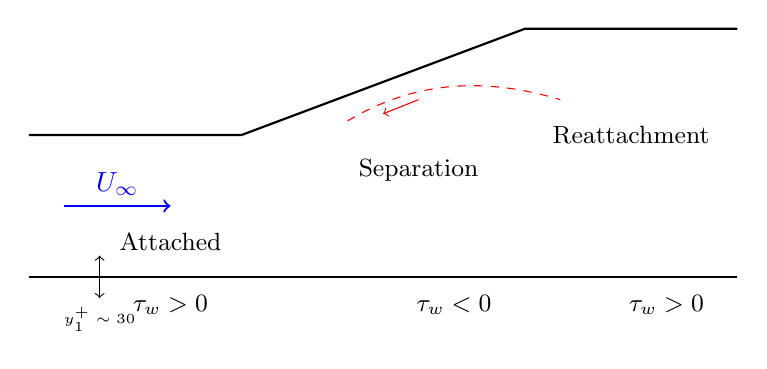
\begin{tikzpicture}[scale=0.9]
        % Channel walls
        \draw[thick] (0,0) -- (10,0);
        \draw[thick] (0,2) -- (3,2) -- (7,3.5) -- (10,3.5);

        % Flow direction
        \draw[->, thick, blue] (0.5,1) -- (2,1) node[midway, above] {$U_\infty$};

        % Separation bubble
        \draw[dashed, red] (4.5,2.2) .. controls (5.5,2.8) and (6.5,2.8) .. (7.5,2.5);
        \draw[->, red, thin] (5.5,2.5) -- (5,2.3);

        % Labels
        \node at (2,0.5) {\small Attached};
        \node at (5.5,1.5) {\small Separation};
        \node at (8.5,2) {\small Reattachment};

        % y+ annotation
        \draw[<->, thin] (1,-0.3) -- (1,0.3);
        \node at (1,-0.6) {\tiny $y^+_1 \sim 30$};

        % tau_w annotations
        \node at (2,-0.4) {\small $\tau_w > 0$};
        \node at (6,-0.4) {\small $\tau_w < 0$};
        \node at (9,-0.4) {\small $\tau_w > 0$};
    \end{tikzpicture}
    \caption{Schematic of flow through an asymmetric diffuser, illustrating attached flow, separation, recirculation, and reattachment. Classical wall functions fail in the separation and recirculation regions where $\tau_w \leq 0$.}
    \label{fig:diffuser_schematic}
\end{figure}

\section{The Machine Learning Opportunity}
\label{sec:intro_ml_opportunity}

Machine learning offers a fundamentally different approach to wall function modeling. Rather than deriving algebraic relationships from similarity theory and asymptotic analysis, machine learning models learn directly from data. High-fidelity simulations---Direct Numerical Simulation (DNS) or well-resolved Large Eddy Simulation (LES)---provide training data that captures the full complexity of near-wall turbulence, including the departures from equilibrium that classical theory cannot accommodate.

Neural networks, as universal function approximators, can represent the nonlinear relationships between near-wall flow quantities and wall fluxes without the limiting assumptions of classical theory. A network trained on diverse flow conditions can interpolate (and potentially extrapolate) to conditions not explicitly represented in the training data, guided by the underlying patterns in the physics rather than by prescribed functional forms.

However, purely data-driven approaches face their own challenges. Neural networks may learn spurious correlations that happen to work within the training distribution but fail catastrophically outside it. Without physical constraints, predictions may violate conservation laws, produce non-physical negative shear stresses, or extrapolate wildly in regions where training data is sparse. The generalization problem---ensuring that models trained on canonical flows perform well in practical applications---remains the central challenge of machine learning for turbulence modeling.

This thesis addresses these challenges through a unified framework that combines data-driven learning with physics-informed constraints. The key insight is that physics knowledge can be incorporated at multiple levels: in the selection and construction of input features, in the architecture of the neural network itself, and in the loss function used during training. By encoding physical principles at each of these levels, we create models that are both flexible enough to learn from data and constrained enough to respect fundamental physics.

\section{Three Approaches to Physics-Informed Learning}
\label{sec:intro_three_approaches}

This thesis develops and compares three complementary methods for incorporating physics knowledge into neural network wall functions. Each method operates at a different level of the machine learning pipeline, and together they provide a comprehensive framework for physics-informed wall function modeling.

\subsection{Method A: Physics-Encoded Input Features}

The first approach encodes physics in the \textit{input representation}. Rather than providing the neural network with raw simulation outputs (velocity components, pressure, temperature at mesh points), we construct non-dimensional features that respect the scaling laws of turbulent boundary layers.

Classical wall function theory teaches us that the relevant variables are wall-scaled quantities: $y^+ = y u_\tau / \nu$, $u^+ = u / u_\tau$, and similar dimensionless groups. These scalings collapse boundary layer data across Reynolds numbers, suggesting that neural networks should receive inputs in these natural coordinates.

We extend this idea to construct a library of 58 physics-based features including:
\begin{itemize}
    \item Wall-scaled distances and velocities ($y^+$, $u^+$, $v^+$)
    \item Pressure gradient terms ($p^+_x = \nu / (\rho u_\tau^3) \cdot \partial p / \partial x$)
    \item Velocity gradient and curvature quantities
    \item Thermal equivalents ($T^+$, $y^+_T$ based on thermal friction velocity)
    \item Deformation tensor invariants
\end{itemize}

Chapter~\ref{chap:physics_features} demonstrates that this physics-encoded input representation enables generalization across Reynolds numbers and achieves accuracy comparable to much larger sets of primitive variables.

\subsection{Method B: Physics-Guided Network Architecture}

The second approach investigates what neural networks learn \textit{internally} when trained on primitive inputs. Even without explicit physics encoding in the inputs, neural networks must construct internal representations to solve the wall function prediction problem. Do these representations correspond to physically meaningful quantities?

Through systematic correlation analysis between hidden layer neuron activations and physics-based features, we find that networks spontaneously discover physics-relevant quantities. Neurons in trained networks correlate strongly with $y^+$, $\ln(y^+)$, and pressure gradient scalings---precisely the quantities that classical wall function theory identifies as important.

Most remarkably, certain features emerge across network architectures of different sizes. A network with 8 hidden neurons and one with 32 hidden neurons both develop neurons correlated with wall-scaled distance. This \textit{architecture invariance} suggests that these features are fundamental to the learning problem, not artifacts of particular network configurations.

Chapter~\ref{chap:neurons} explores these findings, validating the physics-based input design of Method A while revealing the implicit physics learning capabilities of neural networks.

\subsection{Method C: Physics-Constrained Loss Functions}

The third approach encodes physics in the \textit{training objective}. Standard supervised learning minimizes prediction error on training data, but nothing prevents the network from learning solutions that violate physical conservation laws. Physics-Informed Neural Networks (PINNs) address this by adding physics residuals to the loss function:
\begin{equation}
    \mathcal{L} = \mathcal{L}_{\text{data}} + \lambda_{\text{physics}} \mathcal{L}_{\text{physics}}
    \label{eq:pinn_loss_intro}
\end{equation}

For wall functions, we develop a local stencil-based PINN that evaluates conservation law residuals on the same near-wall stencil used for input features. The physics loss penalizes violations of:
\begin{itemize}
    \item Streamwise momentum conservation
    \item Wall-normal momentum (including buoyancy)
    \item Energy conservation
    \item Mass conservation (incompressibility)
\end{itemize}

Unlike global PINNs that require automatic differentiation over entire computational domains, this local approach maintains computational efficiency while enforcing physics constraints where they matter most: in the near-wall region.

Chapter~\ref{chap:pinn} develops this approach and characterizes the trade-off between fitting accuracy and physical consistency.

\subsection{Complementary Methods}

These three methods are not mutually exclusive; they address physics encoding at different stages of the machine learning pipeline:

\begin{center}
\begin{tabular}{|l|l|l|}
    \hline
    \textbf{Method} & \textbf{Stage} & \textbf{Physics Mechanism} \\
    \hline
    A: Physics Inputs & Data preparation & Non-dimensional features \\
    B: Physics Architecture & Model design & Implicit feature discovery \\
    C: Physics Loss & Training objective & Conservation constraints \\
    \hline
\end{tabular}
\end{center}

A comprehensive wall function model might combine all three: physics-encoded inputs, architectures designed to facilitate physics discovery, and loss functions that enforce conservation. The experimental chapters of this thesis evaluate each method independently to understand their individual contributions before considering combinations.

\section{Research Questions}
\label{sec:intro_questions}

This thesis addresses five specific research questions:

\textbf{RQ1: Can machine learning models predict wall shear stress and heat flux accurately across diverse flow conditions?}
This baseline question establishes whether neural networks can learn the wall function mapping at all, and if so, what accuracy is achievable with different input representations and architectures.

\textbf{RQ2: Do physics-based input features improve generalization compared to primitive variables?}
If networks can learn equally well from primitives and from physics features, the additional effort of computing physics-based inputs may not be justified. Conversely, if physics features enable better generalization, they provide a concrete prescription for feature engineering in wall function applications.

\textbf{RQ3: Do neural networks discover physics-based features spontaneously when trained on primitives?}
This question probes the relationship between Methods A and B. If networks discover physics features internally, it validates the importance of these features while suggesting that explicit encoding may not be strictly necessary.

\textbf{RQ4: Does physics-constrained training improve extrapolation to conditions outside the training distribution?}
Method C sacrifices some in-distribution accuracy for physical consistency. The critical question is whether this trade-off pays off when models encounter flows not represented in training data.

\textbf{RQ5: Can ML wall functions be deployed in production CFD codes and outperform classical approaches?}
Academic demonstrations on test sets must ultimately translate to practical utility. This question addresses the engineering viability of the proposed approaches.

\section{Research Objectives}
\label{sec:intro_objectives}

This thesis pursues four interconnected objectives that structure the experimental chapters:

\textbf{Objective 1: Develop a systematic methodology for generating training data.}
High-quality training data is the foundation of any machine learning approach. We develop a dual-mesh methodology that pairs fine-mesh (wall-resolved) simulations with coarse-mesh simulations of the same flow. The fine mesh provides ground-truth wall shear stress and heat flux; the coarse mesh provides the input features that a deployed model would have access to. This approach generates naturally-paired training data across 244 configurations spanning attached and separated flows.

\textbf{Objective 2: Design physics-informed input features.}
Classical wall functions succeed because they use the right non-dimensional variables: $y^+$, $u^+$, and similar quantities that collapse boundary layer profiles across Reynolds numbers. We develop a library of 58 physics-based features derived from the near-wall stencil data, encoding quantities like local velocity gradients, pressure gradients, curvature terms, and thermal variables in wall-scaled and non-dimensional forms. These features provide the neural network with inputs that respect the scaling laws of turbulent boundary layers.

\textbf{Objective 3: Investigate physics-guided architectures and training.}
Beyond input features, physical knowledge can be encoded in the network architecture and training procedure. We investigate whether neural networks spontaneously discover physics-based features in their hidden layers, and we develop physics-constrained loss functions that penalize violations of conservation laws during training.

\textbf{Objective 4: Integrate trained models into production CFD solvers.}
Academic machine learning research often stops at demonstrating accuracy on test sets. We complete the engineering loop by implementing trained models as boundary conditions in OpenFOAM, validating performance on benchmark cases beyond the training distribution, and comparing against classical wall functions in both two-dimensional and three-dimensional configurations.

\section{Thesis Contributions}
\label{sec:intro_contributions}

This thesis makes the following contributions to the field of machine learning for computational fluid dynamics:

\begin{enumerate}
    \item \textbf{A dual-mesh training data generation methodology} that systematically produces paired input-output data for wall function learning across diverse flow conditions. The resulting dataset of 25,485 training samples spans Reynolds numbers 8,000--24,000 and geometric configurations from mild acceleration to strong separation.

    \item \textbf{A physics-based feature library} comprising 58 non-dimensional quantities derived from the near-wall stencil. Systematic experiments demonstrate that a core subset of 11 physics features achieves accuracy comparable to much larger primitive-variable input sets, while providing interpretability advantages.

    \item \textbf{Evidence for architecture-invariant feature discovery}, showing that neural networks trained on primitive inputs spontaneously develop hidden layer neurons correlated with physics-based quantities like $y^+$, $\ln(y^+)$, and pressure gradient scalings. This finding validates the physics-based input design and suggests that certain features emerge naturally from the learning problem.

    \item \textbf{A local stencil-based Physics-Informed Neural Network} that enforces conservation laws (momentum, energy, mass) as soft constraints during training. Unlike global PINNs that require automatic differentiation over entire domains, this approach evaluates physics residuals on the same local stencil used for predictions, maintaining computational efficiency while improving physical consistency.

    \item \textbf{A complete OpenFOAM integration} including C++ boundary condition implementation, Python-to-C++ model export infrastructure, and validation on benchmark cases including backward-facing steps and periodic hills.
\end{enumerate}

\section{Scope and Limitations}
\label{sec:intro_scope}

To maintain focus and depth, this thesis adopts specific boundaries on the problems addressed:

\textbf{Flow regimes.} We consider incompressible, low-Mach-number flows with Reynolds numbers in the range 8,000--24,000. While the methodology extends in principle to compressible flows and higher Reynolds numbers, validation is limited to the incompressible regime.

\textbf{Turbulence modeling.} All simulations use Reynolds-Averaged Navier-Stokes (RANS) equations with the $k$-$\omega$ SST turbulence model. The wall functions developed here could be adapted for Large Eddy Simulation, but LES-specific considerations (subgrid scale modeling near walls) are not addressed.

\textbf{Geometry.} Training data comes from two-dimensional channel, diffuser, and nozzle configurations. Validation includes two-dimensional benchmark cases (backward-facing step, periodic hills) and preliminary three-dimensional results, but comprehensive three-dimensional validation remains future work.

\textbf{Thermal coupling.} We consider passive scalar transport with fixed wall temperatures. Conjugate heat transfer, radiative effects, and strongly-coupled thermal-fluid interactions are outside the scope.

\textbf{Transient effects.} All simulations assume steady-state conditions. Extension to unsteady flows, where temporal history effects may be important, is identified as a direction for future research.

These limitations define the domain within which the thesis results are validated. Extensions beyond these boundaries are discussed in Chapter~\ref{chap:conclusion} as opportunities for future work.

\section{Thesis Outline}
\label{sec:intro_outline}

This thesis is organized as follows:

\textbf{Chapter~\ref{chap:literature}: Literature Review} traces the evolution of wall function modeling from Prandtl's boundary layer theory through modern machine learning approaches. The chapter situates the present work within this intellectual history, identifying the specific gaps that the thesis addresses.

\textbf{Chapter~\ref{chap:methodology}: Methodology and Structured Data Generation} describes the computational setup, including the dual-mesh approach for generating paired training data, the OpenFOAM simulation configurations, and the post-processing pipeline that constructs stencil-based inputs from raw simulation outputs.

\textbf{Chapter~\ref{chap:baseline}: Data-Driven Velocity and Thermal Wall Functions} presents the baseline machine learning approach: fully-connected neural networks trained on primitive flow variables to predict wall shear stress and heat flux. This chapter establishes the achievable accuracy and identifies limitations that motivate the physics-informed extensions.

\textbf{Chapter~\ref{chap:physics_features}: Non-Dimensional Feature Library} develops the library of 58 physics-based input features and systematically compares performance against primitive-variable inputs (Method A). The chapter identifies a core set of features that balance accuracy, interpretability, and computational cost.

\textbf{Chapter~\ref{chap:neurons}: Physics-Guided Hidden Layers} investigates what neural networks learn internally when trained on primitive inputs (Method B). Through correlation analysis between hidden layer activations and physics-based features, the chapter demonstrates that networks discover wall-scaled quantities even without explicit physics encoding.

\textbf{Chapter~\ref{chap:pinn}: Physics-Constrained Learning} develops and evaluates the local stencil-based PINN approach (Method C), incorporating conservation law residuals into the training loss function. The chapter characterizes the trade-off between fitting accuracy and physical consistency.

\textbf{Chapter~\ref{chap:separation}: Identification of Flow Separation} addresses the distinct challenge of detecting separated regions, where classical wall functions fail most severely. The chapter develops classifiers that distinguish attached from separated flow based on the same stencil inputs.

\textbf{Chapter~\ref{chap:openfoam}: OpenFOAM Integration and Validation} presents the production implementation, including C++ boundary condition code, model export utilities, and comprehensive validation on benchmark geometries beyond the training distribution.

\textbf{Chapter~\ref{chap:conclusion}: Conclusion and Future Work} summarizes the contributions, discusses limitations, and outlines directions for future research including extension to higher Reynolds numbers, three-dimensional flows, and unsteady applications.

\section{Chapter Summary}
\label{sec:intro_summary}

Turbulent flow simulation requires accurate treatment of the near-wall region where steep gradients develop. Classical wall functions, while computationally efficient, fail under conditions of adverse pressure gradients, flow separation, and strong thermal coupling---precisely the conditions of greatest engineering interest. The economic implications span industries from aerospace to building ventilation, motivating sustained research into improved wall function models.

Machine learning offers the potential to learn wall function models directly from high-fidelity data, but purely data-driven approaches risk learning spurious correlations that fail outside the training distribution. This thesis develops a physics-informed machine learning framework that combines the flexibility of neural networks with the constraints of physical law. Three complementary methods encode physics knowledge at different stages: in the input features (Method A), in the network architecture through implicit discovery (Method B), and in the training loss function (Method C).

The resulting models are integrated into OpenFOAM for practical CFD applications, demonstrating improved performance over classical approaches across a range of benchmark configurations. The following chapters develop this framework systematically, from data generation through production deployment, contributing both methodological advances and practical tools to the field of machine learning for computational fluid dynamics.

\end{document}
